\documentclass{article}
\usepackage[utf8]{inputenc}
\usepackage[english]{babel}
\usepackage[]{amsthm} 
\usepackage[]{amssymb} 
\usepackage{amsmath}
\DeclareMathOperator{\domain}{dom}
\usepackage{graphicx}
\usepackage{hyperref}
\usepackage{comment}
\usepackage[dvipsnames]{xcolor}
\usepackage[thinc]{esdiff}
\usepackage{tcolorbox}
\usepackage{cancel}
\usepackage{graphicx}
\usepackage{float}
\graphicspath{ {./HW2_images/} }
\newtheorem*{theorem}{Theorem}
\newenvironment{solution}
  {\renewcommand\qedsymbol{$\blacksquare$}\begin{proof}[Solution]}
  {\end{proof}}

\newenvironment{claim}[1]{\par\noindent\underline{Claim:}\space#1}{}
\newenvironment{claimproof}[1]{\par\noindent\underline{Proof:}\space#1}{}
\DeclareMathOperator{\interior}{int}


\title{Optimization Algorithms: HW2}
\author{Lo Chun, Chou \\ R13922136}
\date\today

\begin{document}
\setlength{\parindent}{0pt}
\maketitle 

\tcbset{
    greenbox/.style={
        colback=SpringGreen!20,
        colframe=SpringGreen!80,
        coltitle=black,
        sharp corners
    },
    bluebox/.style={
        colback=SkyBlue!20,
        colframe=SkyBlue!80,
        coltitle=black,
        sharp corners
    },
    yellowbox/.style={
        colback=yellow!10,
        colframe=yellow!80,
        coltitle=black,
        sharp corners
    }
}

\section*{1}

We're given the following problem:

\begin{align*}
    x_{\star} \in \arg\min_{x \in \Delta_d} f(x), \qquad f(x) = -\sum_{i=1}^n w_i \log \langle a_i, x \rangle
\end{align*}

where:

\begin{enumerate}
    \item 
    \begin{align*}
        x \in \Delta_d = \{ x \in \mathbb{R}^d \mid x[i] \geq 0, \sum_{i=1}^d x[i] = 1 \} \ (\text{probabilit`y simplex})
    \end{align*}
    \item 
    \begin{align*}
        w_i \in \mathbb{R}, \ w_i > 0, \ \sum_{i=1}^n w_i = 1
    \end{align*}
    \item 
    \begin{align*}
        &a_i \in \mathbb{R}^d, \ 
        a_i =
        \begin{bmatrix}
            a_i[1] \\
            a_i[2] \\
            \vdots \\
            a_i[d]
        \end{bmatrix}, \\ 
        &a_i[j] \geq 0 \ \forall i = 1, \dots, n, \ j = 1, \dots, d \\
        &a_i \neq 0 \ \forall i = 1, \dots, n
    \end{align*}
\end{enumerate}

We're asked to show that:

$f$ is $1$-smooth relative to the log-barrier, which is defined as:

\begin{align*}
    h(x) = -\sum_{i=1}^d \log x[i]
\end{align*}

\begin{solution}
%     By lecture slide 4, p.13, we have the definition of relative smoothness:
    
%     \begin{tcolorbox}[bluebox]
%         A function $f$ is $L$-smooth relative to a convex function $h$ for some $L > 0$ if:
%         \begin{align*}
%             f(y) \leq f(x) + \langle \nabla f(x), y - x \rangle + L D_h(y, x)
%         \end{align*}
%     \end{tcolorbox}
% \end{solution}

% Therefore, we need to prove that the following condition holds:

% \begin{align*}
%     -\sum_{i=1}^n w_i \log \langle a_i, y \rangle 
%     \leq -\sum_{i=1}^n w_i \log \langle a_i, x \rangle + \langle \nabla f(x), y - x \rangle + L \{ h(y) - \left[h(x) + \langle \nabla h(x), (y - x) \rangle \right]\}
% \end{align*}

By the following proposition
\footnote{\textit{Relative Smooth Convex Optimization by First-Order Methods, and Applications}, MIT Lecture Notes, available at: \url{https://dspace.mit.edu/bitstream/handle/1721.1/120867/16m1099546.pdf}, accessed: May.~9, 2025, p.~336.}:
\begin{figure}[H]
    \centering
    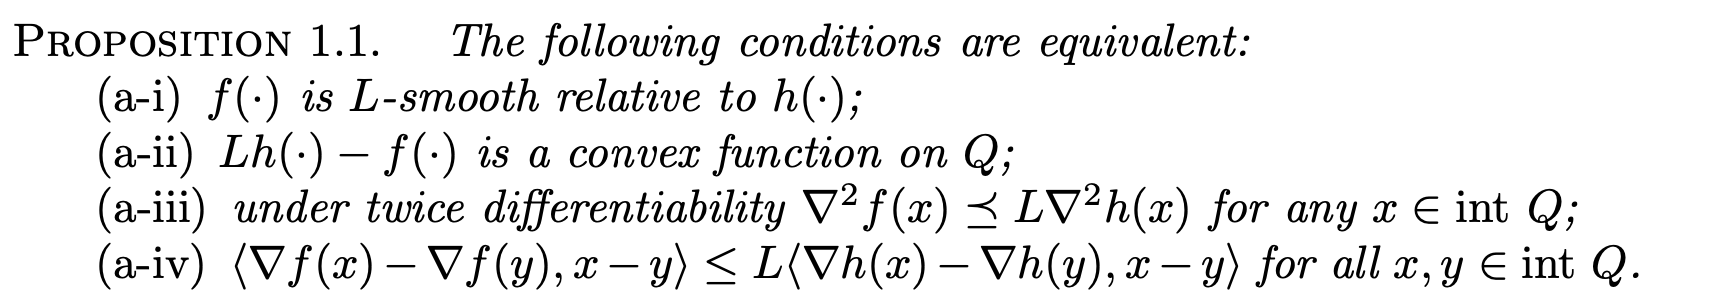
\includegraphics[width = 0.8\textwidth]{proposition_1.1}
\end{figure}
\bigskip

we could prove the required condition (which is (a-i), with $L = 1$) 
by proving its equivalent condition (a-iii, with $L = 1$).
\bigskip

First calculate $\nabla f(x)$:

\begin{align*}
    \nabla f(x) 
    &= \frac{d}{dx} \left( -\sum_{i=1}^n w_i \log \langle a_i, x \rangle \right) \\
    &= -\sum_{i=1}^n w_i \cdot \frac{d}{dx} \left( \log \langle a_i, x \rangle \right) \\
    &= -\sum_{i=1}^n w_i \cdot \left(\frac{a_i}{\langle a_i, x \rangle}\right) \\
    &= -\sum_{i=1}^n w_i \frac{a_i}{\langle a_i, x \rangle}
\end{align*}

Then the Hessian of $f$ is:

\begin{align*}
    \nabla^2 f(x) 
    &= \frac{d}{dx} \left( -\sum_{i=1}^n w_i \frac{a_i}{\langle a_i, x \rangle} \right) \\
    &= -\sum_{i=1}^n w_i \cdot \frac{d}{dx} \left( \frac{a_i}{\langle a_i, x \rangle} \right) \\
    &= -\sum_{i=1}^n w_i \cdot \left( \frac{a_i }{\langle a_i, x \rangle^2} a_i^T\right) \\
\end{align*}

Expanding the expression and writing in another form, we have:

\begin{align*}
    \nabla^2 f(x) 
    &= -\sum_{i=1}^n \frac{w_i}{\langle a_i, x \rangle^2} a_i a_i^T \tag{1}
\end{align*}

Then we shall do the same to $h(x)$

\begin{align*}
    \nabla h(x) 
    &= \frac{d}{dx} \left( -\sum_{i=1}^d \log x[i] \right) \\
    &= 
    \begin{bmatrix}
        -\frac{1}{x[1]} \\
        -\frac{1}{x[2]} \\
        \vdots \\
        -\frac{1}{x[d]}
    \end{bmatrix}
\end{align*}

Then $\nabla^2 h(x)$ is:

\begin{align*}
    \nabla^2 h(x) 
    &= \nabla 
    \begin{bmatrix}
        -\frac{1}{x[1]} \\
        -\frac{1}{x[2]} \\
        \vdots \\
        -\frac{1}{x[d]}
    \end{bmatrix} \\
    &= 
    \begin{bmatrix}
        &\frac{d}{dx[1]} \left( -\frac{1}{x[1]} \right) &\frac{d}{dx[2]} \left( -\frac{1}{x[1]} \right) &\cdots &\frac{d}{dx[d]} \left( -\frac{1}{x[1]} \right) \\
        &\frac{d}{dx[1]} \left( -\frac{1}{x[2]} \right) &\frac{d}{dx[2]} \left( -\frac{1}{x[2]} \right) &\cdots &\frac{d}{dx[d]} \left( -\frac{1}{x[2]} \right) \\
        &\vdots & & \ddots & \vdots \\
        &\frac{d}{dx[1]} \left( -\frac{1}{x[d]} \right) &\frac{d}{dx[2]} \left( -\frac{1}{x[d]} \right) &\cdots &\frac{d}{dx[d]} \left( -\frac{1}{x[d]} \right)
    \end{bmatrix} \\
    &=
    \begin{bmatrix}
        \frac{1}{x[1]^2} & 0 & \cdots & 0 \\
        0 & \frac{1}{x[2]^2} & \cdots & 0 \\
        \vdots & & \ddots & \vdots \\
        0 & 0 & \cdots & \frac{1}{x[d]^2}
    \end{bmatrix} \tag{2}
\end{align*}

Observe $\nabla^2 f(x)$ in $(1)$, since we're given $w_i > 0$, $x \in \Delta_d$, $a_i \neq 0$, 
and with proposition (a-iii) only requires dealing with $\interior \Delta_d$,
we can guarantee $x[i] > 0$, 
so the scalar $\frac{w_i}{\langle a_i, x \rangle^2} > 0$.
\bigskip

Also, we knew that for any $a_i \neq 0$, $a_i a_i^T$ is positive semidefinite,
thus, each term in the summation is positive semidefinite, 
by summing up the $n$ terms and adding a negative sign,
we have $\nabla^2 f(x) \preceq 0$ as follows:

\begin{align*}
    \nabla^2 f(x) 
    = -\sum_{i=1}^n \frac{w_i}{\langle a_i, x \rangle^2} a_i a_i^T \preceq 0
\end{align*}



% We then first show that $\nabla^2 f(x)$ is symmetric, and $\nabla^2 h(x)$ is positive definite,
% in order to use the following generalized Rayleigh quotient to prove that $\nabla^2 f(x) \preceq L \nabla^2 h(x)$:

% \begin{figure}[H]
%     \centering
%     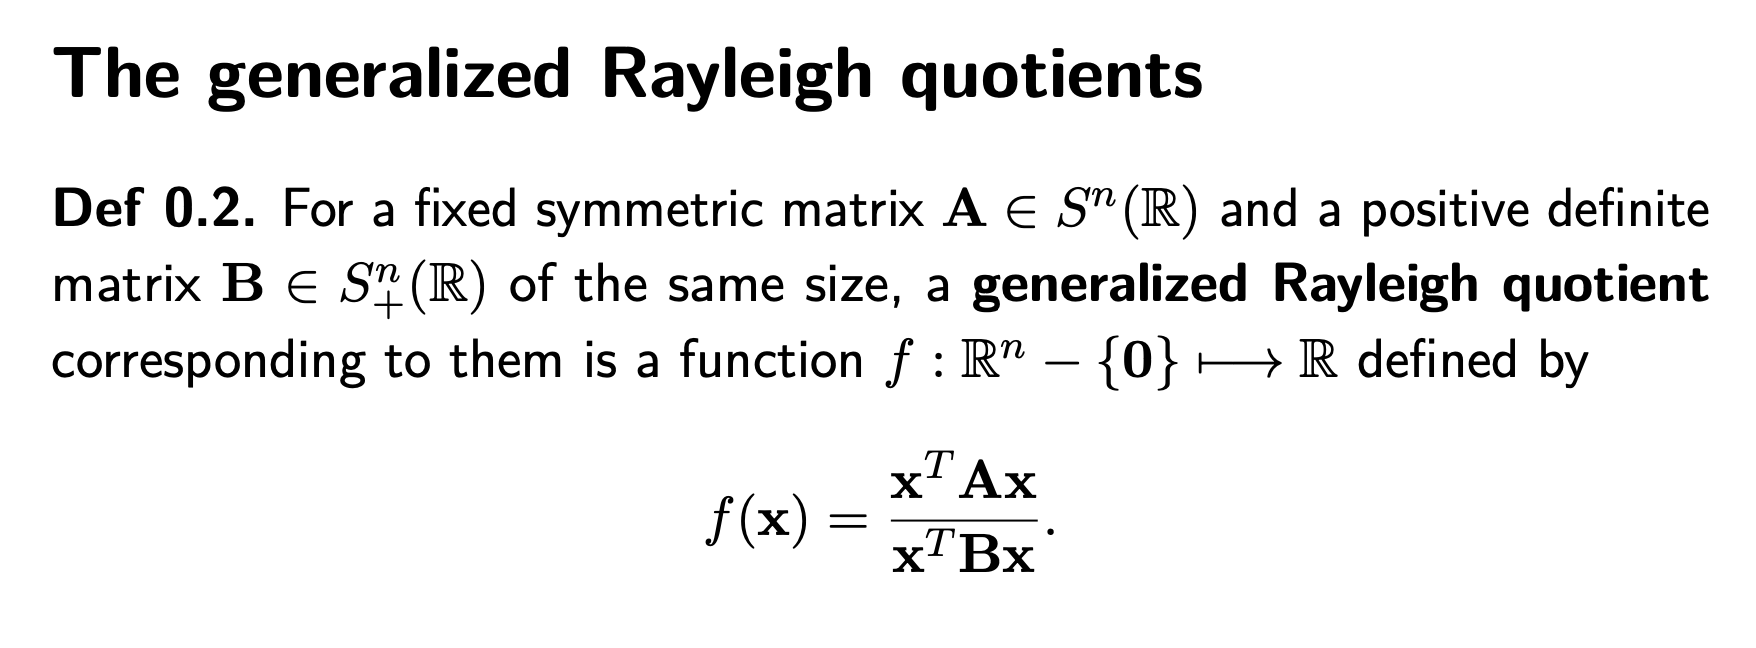
\includegraphics[width = 0.8\textwidth]{generalized_rayleigh_quotients.png}
% \end{figure}

% By our previous calculation, we have:

% \begin{align*}
%     \nabla^2 f(x) = -\sum_{i=1}^n \left( \frac{w_i}{\langle a_i, x \rangle^2} a_i a_i^T\right)
% \end{align*}

% Since $a_i a_i^T$ is symmetric, and multiplying a scalar $\frac{w_i}{\langle a_i, x \rangle^2}$, 
% summing up symmetric matrices also results in a symmetric matrix,
% we have $\nabla^2 f(x)$ is symmetric.
% \bigskip

Then, since $\nabla^2 h(x)$ is a diagonal matrix, and we're given that $x[i] \geq 0$,
same as above, with proposition (a-iii) only requires dealing with $\interior \Delta_d$,
we can guarantee $x[i] > 0$ (so for each $\frac{1}{x[i]}$), and $\nabla^2 h(x)$ is positive definite.
\bigskip

Therefore, we have:

\begin{align*}
    \nabla^2 f(x) \preceq 1 \cdot \nabla^2 h(x) \quad \text{ for any } x \in \interior \Delta_d
\end{align*}

which means that (a-iii) is proved, 
and its equivalent condition (a-i) is also proved, and we have:

\begin{align*}
    f \text{ is } 1\text{-smooth relative to the log-barrier } h
\end{align*}



% Therefore, by letting $A = \nabla^2 f(x)$ and $B = \nabla^2 h(x)$,
% with $z \in \mathbb{R}^d - \{0\}$,
% we define the generalized Rayleigh quotient:

% \begin{align*}
%     R(z) 
%     &= \frac{z^T \nabla^2 f(x) z}{z^T \nabla^2 h(x) z} \\
%     &= \frac{z^T \left( -\sum_{i=1}^n \left( \frac{w_i}{\langle a_i, x \rangle^2} a_i a_i^T\right) \right) z}{-\sum_{i=1}^d \left( \frac{1}{x[i]} z[i]^2\right)} \\
%     &= \frac{\sum_{i=1}^n \left( \frac{w_i}{\langle a_i, x \rangle^2} z^T a_i a_i^T z\right) }{-\sum_{i=1}^d \left( \frac{1}{x[i]} z[i]^2\right)} \\
%     &= \frac{\sum_{i=1}^n \left( \frac{w_i}{\langle a_i, x \rangle^2} \Vert a_i^T z \Vert^2 \right) }{-\sum_{i=1}^d \left( \frac{1}{x[i]} z[i]^2\right)} \\
%     &= \frac{\sum_{i=1}^n \left[ \frac{w_i}{\langle a_i, x \rangle^2} \textcolor{blue}{\left( \sum_{j=1}^d a_i[j] z[j] \right)^2} \right] }{-\sum_{i=1}^d \left( \frac{1}{x[i]} z[i]^2\right)} \\
% \end{align*}

% Using Cauchy-Schwarz inequality in $\mathbb{R}^d$, which is
% \footnote{\textit{Cauchy-Schwarz inequality}, available at: \url{https://en.wikipedia.org/wiki/Cauchy–Schwarz_inequality}, accessed: May.~10, 2025.}:

% \begin{align*}
%     \left( \sum_{i=1}^d u_i v_i \right)^2 \leq \left( \sum_{i=1}^d u_i^2 \right) \left( \sum_{i=1}^d v_i^2 \right)
% \end{align*}

% we have:

% \begin{align*}
%     \left( \sum_{i=1}^d a_i[j] z[j] \right)^2
%     \leq \left( \sum_{i=1}^d a_i[j]^2 \right) \left( \sum_{i=1}^d z[j]^2 \right)
% \end{align*}

% Thus we can bound the previous expression and get:

% \begin{align*}
%     \frac{\sum_{i=1}^n \left[ \frac{w_i}{\langle a_i, x \rangle^2} \textcolor{blue}{\left( \sum_{j=1}^d a_i[j] z[j] \right)^2} \right] }{-\sum_{i=1}^d \left( \frac{1}{x[i]} z[i]^2\right)}
%     \leq \frac{\sum_{i=1}^n \left[ \frac{w_i}{\langle a_i, x \rangle^2} \textcolor{blue}{\left( \sum_{j=1}^d a_i[j]^2 \right) \left( \sum_{j=1}^d z[j]^2 \right)} \right] }{-\sum_{i=1}^d \left( \frac{1}{x[i]} z[i]^2\right)}
% \end{align*}



\end{solution}

\newpage


Denote the Bregman divergence associated with $h$ as $D_h$, i.e.,

\begin{align*}
    D_h(y, x) = h(y) - \left[h(x) + \langle \nabla h(x), (y - x) \rangle \right]
\end{align*}

Consider solving the optimization problem $(1)$ by the following algorithm:

\begin{itemize}
    \item Let $x_1 = 
    \begin{bmatrix}
        \frac{1}{d} \\
        \vdots \\
        \frac{1}{d}
    \end{bmatrix} 
    \in \Delta_d$
    \item For every $t \in \mathbb{N}$, compute:
    \begin{align*}
        x_{t+1} \in \arg\min_{x \in \Delta_d} \left[ \langle \nabla f(x_t), x - x_t \rangle + D_h(x, x_t) \right]
    \end{align*}
\end{itemize}

Note: I use 
$\begin{bmatrix}
    \frac{1}{d} \\
    \vdots \\
    \frac{1}{d}
\end{bmatrix}$ 
to represent the vector $(1/d, \dots, 1/d)$ (which is the notation used in the HW spec) in the following solution.

\section*{2}

Show that for any $x \in \Delta_d$ and $0 \leq \alpha < 1$,

\begin{align*}
    f(x_\alpha) \leq f(x) + \frac{\alpha}{1 - \alpha}, \quad \text{where} \ x_\alpha 
    = (1 - \alpha) x + \alpha 
    \begin{bmatrix}
        \frac{1}{d} \\
        \vdots \\
        \frac{1}{d}
    \end{bmatrix}
\end{align*}

\begin{solution}
From the previous subproblem, we knew that $f$ is $1$-smooth relative to the log-barrier, so we have:

\begin{align*}
    f(y) \leq f(x) + \langle \nabla f(x), y - x \rangle + D_h(y, x) \quad \forall x, y \in \interior \Delta_d
\end{align*}

To bound $f(x_\alpha)$, we first show that $x_\alpha \in \interior \Delta_d$, 
and then let $y = x_\alpha, \ x = x$ so that we would have:

\begin{align*}
    f(x_\alpha) \leq f(x) + \langle \nabla f(x), x_\alpha - x \rangle + D_h(x_\alpha, x)
\end{align*}

By the definition of $x_\alpha$, we knew that it is the convex combination of $x$ and $\begin{bmatrix}
    \frac{1}{d} \\
    \vdots \\
    \frac{1}{d}
\end{bmatrix}$, 
where $x \in \Delta_d$ and $\begin{bmatrix}
    \frac{1}{d} \\
    \vdots \\
    \frac{1}{d}
\end{bmatrix} = x_1 \in \Delta_d$ as stated in the algorithm.
\bigskip
Also, for each element in $x_\alpha$, we have:

\begin{align*}
    x_\alpha[i] = (1 - \alpha) x[i] + \alpha \left( \frac{1}{d} \right) \qquad \forall i = 1, \dots, d
\end{align*}

Since $x[i] \geq 0$ and $\alpha$ is strictly smaller than $1$,
consider the case that $0 < \alpha < 1$, then we have $x_\alpha[i] > 0$ for all $i = 1, \dots, d$.
For $\alpha = 0$, we have $x_\alpha[i] = x[i] \geq 0$ for all $i = 1, \dots, d$,
\textcolor{red}{and since in order to use the previous inequality, we need $x \in \interior \Delta_d$,
thus each $x[i]$ is strictly positive, so we have $x_\alpha \in \interior \Delta_d$ 
for $\alpha = 0$ (and also for $0 < \alpha < 1$).
}
\bigskip

\textcolor{red}{
$\rightarrow$ need to be true for all $x \in \Delta_d$
}


\bigskip

Then, we have:

\begin{align*}
    f(x_\alpha) \leq f(x) + \langle \nabla f(x), x_\alpha - x \rangle + D_h(x_\alpha, x)
\end{align*}

To further simplify, we have:

\begin{align*}
    x_\alpha - x 
    = \left[ (1 - \alpha) x + \alpha 
    \begin{bmatrix}
        \frac{1}{d} \\
        \vdots \\
        \frac{1}{d}
    \end{bmatrix}
    \right] - x = \alpha \left[ \begin{bmatrix}
    \frac{1}{d} \\
    \vdots \\
    \frac{1}{d} \end{bmatrix} - x \right]
\end{align*}

So we could expand the following expressions:

\begin{align*}
    \langle \nabla f(x), x_\alpha - x \rangle
    &= \langle -\sum_{i=1}^n w_i \frac{a_i}{\langle a_i, x \rangle}, \alpha \left( \begin{bmatrix}
    \frac{1}{d} \\
    \vdots \\
    \frac{1}{d} \end{bmatrix} - x \right) \rangle \\
    &= - \frac{\alpha}{d} \sum_{i = 1}^n \frac{w_i}{\langle a_i, x \rangle} 
        \left[a_i[1] \cdots a_i[d]\right]
        \begin{bmatrix}
        1 - x[1] \\
        \vdots \\
        1 - x[d]
        \end{bmatrix} \\
    &= - \frac{\alpha}{d} \sum_{i = 1}^n \frac{w_i}{\langle a_i, x \rangle} \left( \sum_{j = 1}^d a_i[j] - \sum_{j = 1}^d a_i[j] x[j] \right) \\
    &= - \frac{\alpha}{d} \sum_{i = 1}^n \frac{w_i}{\sum_{k = 1}^d a_i[k] x[k]} \left( \sum_{j = 1}^d a_i[j] - \sum_{j = 1}^d a_i[j] x[j] \right) \\
    &= - \frac{\alpha}{d} \sum_{i = 1}^n \frac{w_i \sum_{j = 1}^d a_i[j]}{\sum_{k = 1}^d a_i[k] x[k]} + \frac{\alpha}{d} \sum_{i = 1}^n w_i \\
    &= \frac{\alpha}{d} \left( 1 - \sum_{i = 1}^n w_i \sum_{j = 1}^d \frac{a_i[j]}{a_i[j] x[j]} \right) \\
    &= \frac{\alpha}{d} \left( 1 - \sum_{i = 1}^n w_i \sum_{j = 1}^d \frac{1}{x[j]} \right)
    \tag{1}
\end{align*}

By the definition of $D_h$, we have:

\begin{align*}
    D_h(x_\alpha, x) 
    &= h(x_\alpha) - \left(h(x) + \langle \textcolor{Green}{\nabla h(x)}, \textcolor{blue}{(x_\alpha - x)} \rangle \right) \\
    &= h(x_\alpha) - \left(h(x) + \langle
        \textcolor{Green}{\begin{bmatrix}
        -\frac{1}{x[1]} \\
        -\frac{1}{x[2]} \\
        \vdots \\
        -\frac{1}{x[d]}
        \end{bmatrix}}, 
    \textcolor{blue}{\alpha \left( \begin{bmatrix}
        \frac{1}{d} \\
        \vdots \\
        \frac{1}{d}
    \end{bmatrix} - x \right) \rangle} \right) \\
    &= -\sum_{i=1}^d \log x_\alpha[i] - \left( -\sum_{i=1}^d \log x[i] + \langle 
    \begin{bmatrix}
        -\frac{1}{x[1]} \\
        -\frac{1}{x[2]} \\
        \vdots \\
        -\frac{1}{x[d]}
    \end{bmatrix}, \alpha \left( \begin{bmatrix}
        \frac{1}{d} \\
        \vdots \\
        \frac{1}{d}
    \end{bmatrix} - x \right) \rangle \right) \\
    &= -\sum_{i=1}^d \log x_\alpha[i] + \sum_{i=1}^d \log x[i] + \alpha [-\frac{1}{x[1]} \cdots -\frac{1}{x[d]}]
    \begin{bmatrix}
        \frac{1 - dx[1]}{d} \\
        \vdots \\
        \frac{1 - dx[d]}{d}
    \end{bmatrix} \\
    &= \sum_{i = 1}^d (\log x[i] - \log x_\alpha[i]) - \sum_{i = 1}^d \frac{\alpha}{d x[i]} + \alpha d \\
    \tag{2}
\end{align*}

Combining (1) and (2), we have:

\begin{align*}
    &\langle \nabla f(x), x_\alpha - x \rangle + D_h(x_\alpha, x) \\
    &= \frac{\alpha}{d} \left( 1 - \sum_{i = 1}^n w_i \sum_{j = 1}^d \frac{1}{x[j]} \right)
        + \sum_{i = 1}^d (\log x[i] - \log x_\alpha[i]) - \sum_{i = 1}^d \frac{\alpha}{d x[i]} + \alpha d \\
    &= 
\end{align*}
\end{solution}

\section*{3}

\section*{4}

\section*{5}

We need to show that the following function is self-concordant:

\begin{align*}
    \varphi(u) = u - \sum_{i=1}^d \log (u + \nabla f(x_t)[i] + \frac{1}{x_t[i]})
\end{align*}

\begin{solution}


In order to show that $\varphi(u)$ is self-concordant, since $\varphi(u)$ is univariate, 
we can directly use the following definition
\footnote{\textit{Self-concordant function}, available at: \url{https://en.wikipedia.org/wiki/Self-concordant_function\#Univariate_self-concordant_function}, accessed: May.~29, 2025.}:
% \footnote{Y. Nesterov, \textit{Introductory Lectures on Convex Optimization: A Basic Course}, 1st ed., Springer, New York, NY, 2004, p.~161.}:

% \begin{figure}[H]
%     \centering
%     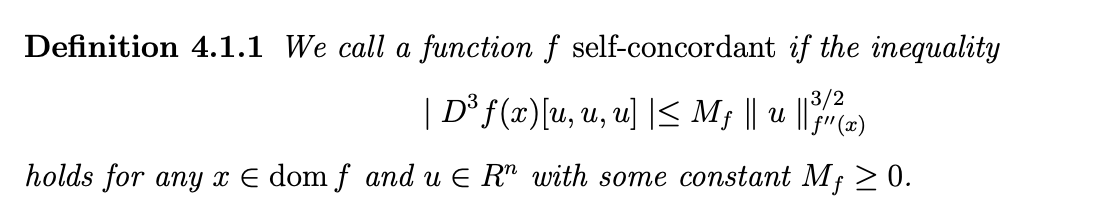
\includegraphics[width = 0.8\textwidth]{self_concordant_def.png}
% \end{figure}

\begin{tcolorbox}[bluebox, title = Self-concordant for univariate functions]
    A function $f: \mathbb{R} \to \mathbb{R}$ is self-concordant on $\mathbb{R}$ if :
    \begin{align*}
        |f'''(x)| \leq 2 f''(x)^{3/2}
    \end{align*}
\end{tcolorbox}

\begin{claim}
    \begin{align*}
        |\varphi'''(u)| \leq 2 \varphi''(u)^{3/2}
    \end{align*}
\end{claim}

\begin{claimproof}
    Let us define:

    \begin{align*}
        y_i := u + \nabla f(x_t)[i] + \frac{1}{x_t[i]}, \qquad \forall i = 1, \dots, d
    \end{align*}

    Then, the original function $\varphi(u)$ can be rewritten as:

    \begin{align*}
        \varphi(u) = u - \sum_{i=1}^d \log y_i = u + \sum_{i=1}^d (-\log y_i)
    \end{align*}

    Now we can compute the dirivatives of $\varphi(u)$:

    \begin{align*}
        \varphi'(u) = 1 - \sum_{i=1}^d \frac{1}{y_i}
    \end{align*}
    
    and the second derivative:

    \begin{align*}
        \varphi''(u) = \sum_{i=1}^d \frac{1}{y_i^2}
    \end{align*}

    and the third derivative:
    
    \begin{align*}
        \varphi'''(u) = -2 \sum_{i=1}^d \frac{1}{y_i^3}
    \end{align*}

    Now we have:
    
    \begin{align*}
        |\varphi'''(u)| &= 2 \sum_{i=1}^d \frac{1}{y_i^3} \\
        \varphi''(u) &= \sum_{i=1}^d \frac{1}{y_i^2} \\
    \end{align*}

    % Then we calculate $2\varphi''(u)^{3/2}$:

    % \begin{align*}
    %     2\varphi''(u)^{3/2} 
    %     &= 2 \left( \sum_{i=1}^d \frac{1}{y_i^2} \right)^{3/2} \\
    %     &=  \\
    % \end{align*}

    In order to let the original definition of $\varphi(u)$ be valid, $y_i \in (0, \infty)$ must hold, 
    thus, if we further define $g(y_i) = - \log y_i$, 
    then 
    
    \begin{align*}
        g : \{y_i \in \mathbb{R} \mid y_i > 0\} \rightarrow \mathbb{R}
    \end{align*}

    , and we have:

    \begin{align*}
        g'(y_i) &= \frac{d}{dy_i} (- \log y_i) = -\frac{1}{y_i} \\
        g''(y_i) &= \frac{d}{dy_i} \left( -\frac{1}{y_i} \right) = \frac{1}{y_i^2} \\
        g'''(y_i) &= \frac{d}{dy_i} \left( \frac{1}{y_i^2} \right) = -\frac{2}{y_i^3} \\
    \end{align*}

    And we have:

    \begin{align*}
        \mid g'''(y_i) \mid = \mid -\frac{2}{y_i^3} \mid = \frac{2}{y_i^3} \leq 2 \left( \frac{1}{y_i^2} \right)^{3/2} = 2 \left(\frac{1}{y_i^3} \right)
    \end{align*}

    Which shows that $g(y_i)$ is self-concordant.
    \bigskip

    Then, using the following property
    \footnote{G. Farina, \textit{Lecture 14A–B: Self-concordant functions}, MIT 6.7220/15.084 — Nonlinear Optimization, Apr.~16--18$^{\text{th}}$ 2024. Available at: \url{https://www.mit.edu/~gfarina/2024/67220s24_L14B_self_concordance/L14.pdf}, p.~4.}:

    \begin{figure}[H]
        \centering
        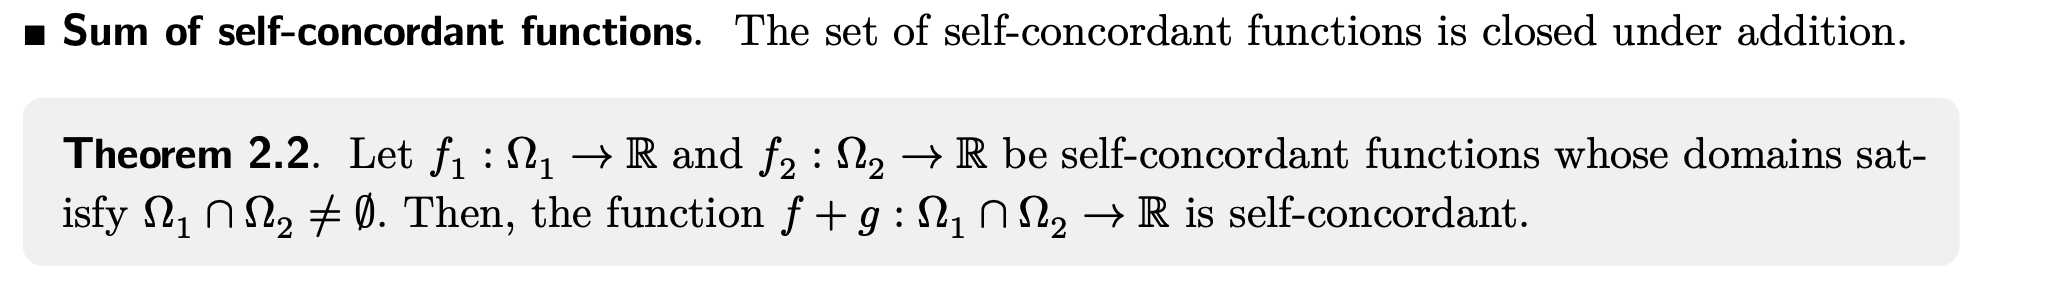
\includegraphics[width = 0.8\textwidth]{sum_self_concordant.png}
    \end{figure}

    Since $g(y_i)$ is self-concordant for all $i = 1, \dots, d$,
    and they have the same domain, so $\bigcap_{i = 1}^d \domain g(y_i) \neq \emptyset$,
    thus, their sum:

    \begin{align*}
        \sum_{i = 1}^d g(y_i) = \sum_{i = 1}^d (-\log y_i)
    \end{align*}

    is also self-concordant.

    \bigskip

    Then, using another property:

    \begin{figure}[H]
        \centering
        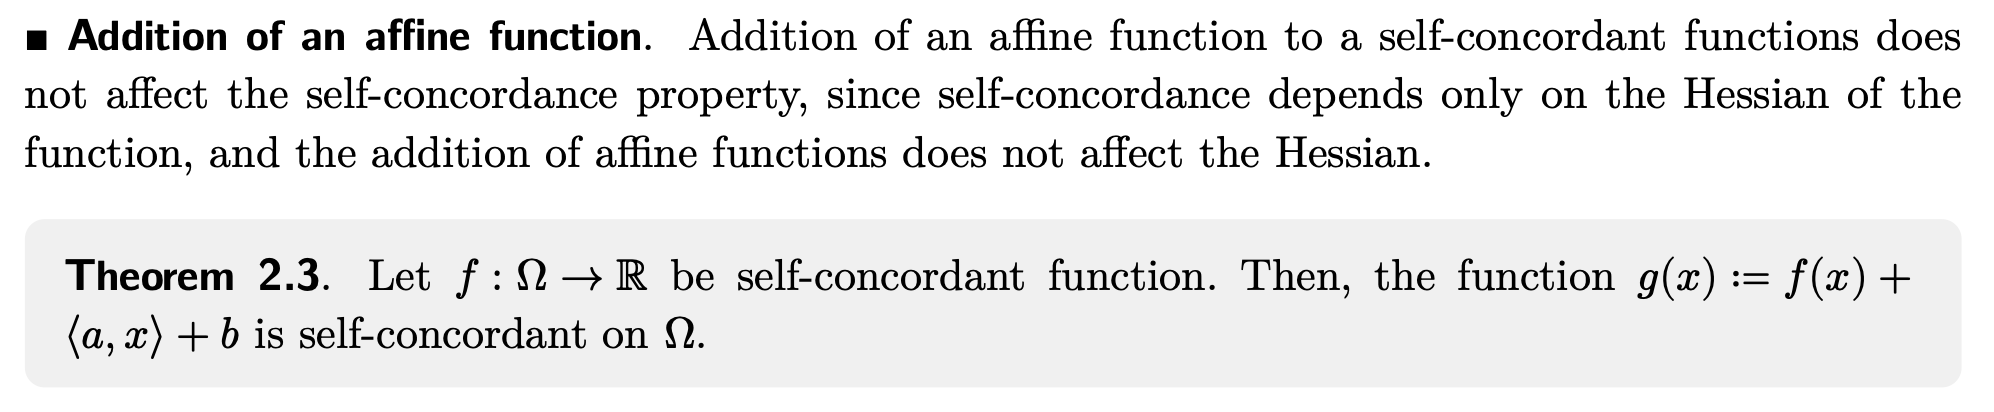
\includegraphics[width = 0.8\textwidth]{affine_self_concordant.png}
    \end{figure}

    If we let $h(u) = u$, then $h$ is an affine function, 
    then our self concordant function $\sum_{i = 1}^d (-\log y_i)$ plussing the affine function $h$:

    \begin{align*}
        \varphi(u) = u + \sum_{i = 1}^d (-\log y_i) 
    \end{align*}

    is also self-concordant.

\end{claimproof}
\end{solution}

\newpage

% Considering the given condition for learning a linear classifier, with data:

% \begin{align*}
%     (x_1, y_1), \dots, (x_n, y_n) \in \mathbb{R}^d \times \{\pm 1\}
% \end{align*}

% , $l_1$-regularized lasso yields the following optimization problem:

% \begin{align*}
%     w_\star \in \arg\min_{w \in \mathbb{R}^d} f(w) + \lambda g(w), \quad \text{with} \ \lambda > 0
% \end{align*}


\section*{6}

We're given that:

\begin{align*}
    g_\mu(w) = \max_{v \in \mathcal{B}_\infty}\langle w, v \rangle - \frac{\mu}{2} \Vert v \Vert^2_2
\end{align*}

where $\mathcal{B}_\infty$ is the unit $l_\infty$ norm ball.
\bigskip

We need to show that $g_\mu$ is differentiable and:

\begin{align*}
    \nabla g_\mu(w) = 
    \begin{cases}
        1 \qquad &\text{if } w[i] \geq \mu \\
        \frac{w[i]}{\mu} \qquad &\text{if } - \mu \leq w[i] \leq \mu \\
        -1 \qquad &\text{if } w[i] < - \mu \\
    \end{cases}
\end{align*}

\begin{solution}
    % Since the dual of $l_\infty$ norm is $l_1$ norm, we have
    % \footnote{S. Boyd, \textit{Convex Optimization}, 1st ed., Cambridge University Press, Cambridge, UK, 2004, p.~637.}:
    % \begin{align*}
    %     \sup \{{w^Tv \mid \Vert v \Vert_\infty \leq 1}\} = \sum_{i = 1}^d \vert w[i] \vert = \Vert w \Vert_1
    % \end{align*}

    By the definition of $l_\infty$ norm, we have:

    \begin{align*}
        \Vert v \Vert_\infty \leq 1 \iff \max_{i = 1, \dots, d} \vert v[i] \vert \leq 1
    \end{align*}

    Then the original $g_\mu(w)$ can be rewritten as:

    \begin{align*}
        g_\mu(w) = \max_{v \in \mathcal{B}_\infty} \sum_{i=1}^d \left( w[i] v[i] - \frac{\mu}{2} v[i]^2\right), \qquad \text{where } \Vert v \Vert_\infty \leq 1
    \end{align*}

    Since to find the $v$ that maximizes the above expression, 
    we can independently find each $v[i]$ that maximizes the component in the summation, 
    so we can further define:

    \begin{align*}
        h_i(w[i]) = \max_{|v[i]| \leq 1} \left( w[i] v[i] - \frac{\mu}{2} v[i]^2 \right)
    \end{align*}

    Then the original $g_\mu(w)$ can be rewritten as:

    \begin{align*}
        g_\mu(w) = \sum_{i=1}^d h_i(w[i])
    \end{align*}

    Now we can prove the differentiability of $g_\mu(w)$ by proving the differentiability of each $h_i(w[i])$.
    Let:

    \begin{align*}
        f_{w[i]}(v[i]) = w[i] v[i] - \frac{\mu}{2} v[i]^2
    \end{align*}

    Since $w[i] v[i]$ is linear in $v[i]$, 
    and the quadratic term $-\frac{\mu}{2} v[i]^2 < 0 \ (\text{for } \mu > 0)$, 
    $f_{w[i]}(v[i])$ is concave in $v[i]$, 
    which means that exists a unique $v^\star[i]$ that maximizes $f_{w[i]}(v[i])$, 
    and we have:

    \begin{align*}
        \frac{d}{dv[i]} f_{w[i]}(v[i]) = w[i] - \mu v[i] = 0 \iff v[i]^* = \frac{w[i]}{\mu}
    \end{align*}

    Thus, if we do not restrict the solution to be in the unit ball, 
    the $v$ that maximizes $\langle w, v \rangle - \frac{\mu}{2} \Vert v \Vert^2_2$ is:

    \begin{align*}
        v^* 
        = \begin{bmatrix}
            \frac{w[1]}{\mu} \\
            \vdots \\
            \frac{w[d]}{\mu}
        \end{bmatrix}
        = \begin{bmatrix}
            v[1] \\
            \vdots \\
            v[d]
        \end{bmatrix}
    \end{align*}

    To further impose the restriction that $\max_{i = 1, \dots, d} \vert v[i] \vert \leq 1$, 
    the optimal $v$ need to satisfy:

    \begin{align*}
        v[i] \in [-1, 1]
    \end{align*}

    Thus, we need to project $v[i]$ to the interval $[-1, 1]$, 
    by the following definition of Euclidean projection
    \footnote{S. Boyd, \textit{Convex Optimization}, 1st ed., Cambridge University Press, Cambridge, UK, 2004, p.~399.}:

    \begin{figure}[H]
        \centering
        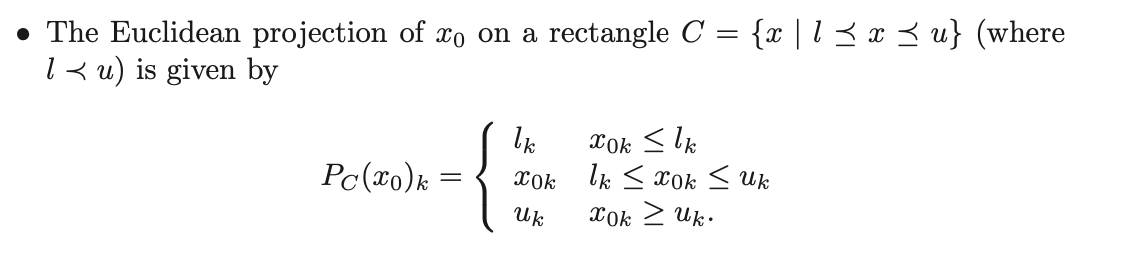
\includegraphics[width = 0.8\textwidth]{euclidean_projection.png}
    \end{figure}

    We have:

    \begin{align*}
        \text{proj}_{[-1, 1]}(v[i]) = \begin{cases}
            -1 \qquad &\text{if } v[i] < -1 \\
            v[i] \qquad &\text{if } -1 \leq v[i] \leq 1 \\
            1 \qquad &\text{if } v[i] > 1 \\
        \end{cases}
    \end{align*}

    or equivalently:

    \begin{align*}
        \text{proj}_{[-1, 1]}\left( \frac{w[i]}{\mu} \right) 
        = v^\star(w[i])
        = \begin{cases}
            -1 \qquad &\text{if } w[i] < - \mu \\
            \frac{w[i]}{\mu} \qquad &\text{if } \vert w[i]\vert \leq \mu \\
            1 \qquad &\text{if } w[i] > \mu \\
        \end{cases} \tag{1}
    \end{align*}

    And this matches the given $\nabla g_\mu(w)[i]$.
    \bigskip

    Then getting back to the part of proving differentiability, we have $h_i(w[i])$:

    \begin{align*}
        h_i(w[i]) 
        &= \max_{|v[i]| \leq 1} \left( w[i] v[i] - \frac{\mu}{2} v[i]^2 \right) \\
        &= \max_{|v[i]| \leq 1} \left(f_{w[i]}(v[i])\right) \\
        &= f_{w[i]}(v^\star(w[i])) \\
        &= w[i] v^\star (w[i]) - \frac{\mu}{2} (v^\star (w[i]))^2 \tag{2}
    \end{align*}

    Consider the three cases of $\text{proj}_{[-1, 1]}(v[i])$ in $(1)$:
    \bigskip

    \begin{itemize}
        \item \underline{Case 1:} $w[i] < - \mu$
        \bigskip

        Then $v^\star(w[i]) = -1$, and by plugging it into $(2)$:
        \begin{align*}
            &h_i(w[i]) = w[i] (-1) - \frac{\mu}{2} (-1)^2 = - w[i] - \frac{\mu}{2} \\
            \rightarrow \ & h_i'(w[i]) = \frac{d}{dw[i]} \left( - w[i] - \frac{\mu}{2} \right) = -1 \\
        \end{align*}

        \item \underline{Case 2:} $- \mu \leq w[i] \leq \mu$
        \bigskip

        Then $v^\star(w[i]) = \frac{w[i]}{\mu}$, and by plugging it into $(2)$:
        \begin{align*}
            &h_i(w[i]) = w[i] \frac{w[i]}{\mu} - \frac{\mu}{2} \left( \frac{w[i]}{\mu} \right)^2 = \frac{w[i]^2}{\mu} - \frac{\mu}{2} \frac{w[i]^2}{\mu^2} = \frac{w[i]^2}{2\mu} \\
            \rightarrow \ & h_i'(w[i]) = \frac{d}{dw[i]} \left( \frac{w[i]^2}{2\mu} \right) = \frac{w[i]}{\mu} \\
        \end{align*}

        \item \underline{Case 3:} $w[i] > \mu$
        \bigskip

        Then $v^\star(w[i]) = 1$, and by plugging it into $(2)$:
        \begin{align*}
            &h_i(w[i]) = w[i] (1) - \frac{\mu}{2} (1)^2 = w[i] - \frac{\mu}{2} \\
            \rightarrow \ & h_i'(w[i]) = \frac{d}{dw[i]} \left( w[i] - \frac{\mu}{2} \right) = 1 \\
        \end{align*}
    \end{itemize}

    Thus, at the boundaries:

    \begin{itemize}
        \item $w[i] = \mu$
        \bigskip

        Left derivative:
        \begin{align*}
            \lim_{w[i] \to \mu^-} h_i'(w[i]) = \lim_{w[i] \to \mu^-} \frac{w[i]}{\mu} = \frac{\mu}{\mu} = 1
        \end{align*}

        Right derivative:
        \begin{align*}
            \lim_{w[i] \to \mu^+} h_i'(w[i]) = 1
        \end{align*}

        \item $w[i] = - \mu$
        \bigskip

        Left derivative:
        \begin{align*}
            \lim_{w[i] \to - \mu^-} h_i'(w[i]) = -1
        \end{align*}

        Right derivative:
        \begin{align*}
            \lim_{w[i] \to - \mu^+} h_i'(w[i]) = \lim_{w[i] \to - \mu^+} \frac{w[i]}{\mu} = \frac{- \mu}{\mu} = -1
        \end{align*}
    \end{itemize}

    And in the interior:

    \begin{align*}
        h_i'(w[i]) 
        &= w[i] \frac{w[i]}{\mu} - \frac{\mu}{2} \left(\frac{w[i]}{\mu}\right)^2 \\
        &= \frac{w[i]^2}{\mu} - \frac{w[i]^2}{2\mu} \\
        &= \frac{w[i]^2}{2\mu}
    \end{align*}

    Which always exists and is unique.
    \bigskip

    Therefore, $h_i(w[i])$ is differentiable, and $g_\mu(w) = \sum_{i=1}^d h_i(w[i])$ is a sum of differentiable functions, 
    so $g_\mu(w)$ is also differentiable.
    
\end{solution}

\section*{7}

We need to further prove that $g_\mu$ is $\frac{1}{\mu}$-smooth.

\begin{solution}

    By the definition in the lecture note
    \footnote{Lecture 4: Mirror Descent, p.~10}, we have:

    \begin{tcolorbox}[bluebox, title = $L$-Smooth]
        We say a differentiable function $f: \mathbb{R}^d \to \mathbb{R}$ is $L$-smooth for some $L > 0$ if:

        \begin{align*}
            f(y) \leq f(x) + \langle \nabla f(x), y - x \rangle + \frac{L}{2} \Vert y - x \Vert_2^2, \qquad \forall x, y \in \mathbb{R}^d
        \end{align*}
    \end{tcolorbox}

    \begin{claim}
        \begin{align*}
            g_\mu(w_1) \leq g_\mu(w_2) + \langle \nabla g_\mu(w_2), w_1 - w_2 \rangle + \frac{1}{2\mu} \Vert w_1 - w_2 \Vert_2^2, \qquad \forall w_1, w_2 \in \mathbb{R}^d
        \end{align*}
    \end{claim}

    \begin{claimproof}
        \begin{align*}
            g_\mu(w_1) 
            &= \max_{v \in \mathcal{B}_\infty} \langle y, v \rangle - \frac{\mu}{2} \Vert v \Vert^2_2 \\
            &= \max_{v \in \mathcal{B}_\infty} \langle x, v \rangle - \frac{\mu}{2} \Vert v \Vert^2_2 + \langle y - x, v \rangle \\
            &= g_\mu(x) + \langle y - x, v \rangle
        \end{align*}
    \end{claimproof}

\end{solution}



\end{document}